\section{Постановка эксперимента}

\subsection{Конфигурация экспериментального стенда}

\subsubsection{Аппаратное обеспечение}

Процессоры 2 x Intel Xeon Platinum 8168 CPU @ 2.7 GHz.
Технология Hyper-Threading отключена для уменьшения нежелательного влияния на время обслуживания заявок в системе \cite{LowLatencyHT}.

Оперативная память: DDR4-2666 128 GiB.

\subsubsection{Программное обеспечение}

Операционная система Red Hat Enterprise Linux Server release 7.8 (Maipo).
Ядро Linux 3.10.0-1127.el7.x86\_64

Компилятор C++ Clang 6.0.1.

Стандартная библиотека C++: libstdc++ 8.1.0.

Библиотека Boost.Interprocess 1.68.0.

\subsection{Конфигурация экспериментальной системы}

Система для проведения эксперимента состоит из двух процессов:
\begin{itemize}
\item Процесс-шлюз отвечает за преобразование заявок из формата внешнего мира во внутренний формат системы и обратно. 
\item Процесс-обработчик совершает некоторые преобразования над заявкой и отправляет результат за пределы системы через процесс-шлюз.
\end{itemize}

Процессы выполняются на двух процессорах, расположенных в разных разъемах на материнской плате физического узла.

Снаружи системы находится симулятор внешнего мира. Он генерирует поток заявок в систему и получает результат обслуживания заявки в системе. Схема взаимодействия процессов в эксперименте представлена на рисунке \ref{chapter41:SystemSchema}.

\begin{figure}[!h]
\caption{Схема взаимодействия процессов в эксперименте}
\label{chapter41:SystemSchema}
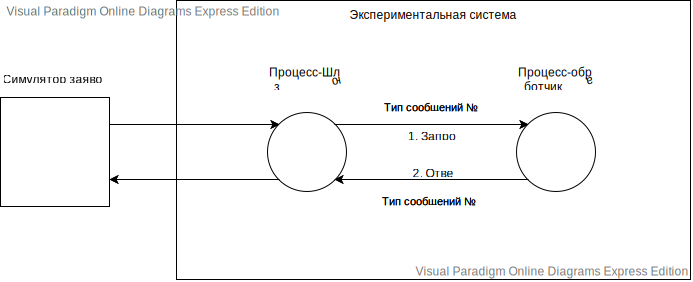
\includegraphics[width=\textwidth]{../../graphics/schemes/SystemSchema}
\end{figure}

В настоящей работе замеряется временная задержка на передачу данных между процессами внутри системы, а именно из процесса-шлюза в процесс-обработчик и обратно (сообщения типа №1 и №2 в запросе и ответе между процессом-шлюзом и процессом обработчиком на рисунке \ref{chapter41:SystemSchema}).

Процессы системы взаимодействуют используют одно соединение, в рамках которого заявки обрабатываются строго последовательно.
Обслуживание включает в себя: прием заявки, выполнение пользовательской логики над заявкой и, если необходимо, отправка ответа.
Временной задержкой на передачу данных в настоящей работе принимается временной промежуток от начала отправки заявки до \textbf{начала обслуживания заявки}. Таким образом, возможен случай, когда во время обслуживания очередной заявки процессом в очереди уже находится следующая заявка, временная задержка на передачу которой, таким образом, увеличится на время обслуживания текущей заявки.

Данный сценарий актуален для процесса-обработчика, в котором обслуживание заявки осуществляется непосредственно в транспортном потоке
В случае с процессом-шлюзом транспортный поток только читает и диспетчеризует асинхронное обслуживание заявки, т.е. не выполняет обслуживание самой заявки.

\textbf{TBD: надо как- то адекватно это описать}
Пользовательская логика процесс-обработчика в среднем отклоняет 25\% заявок, в то время как 75\% заявок отправляются в процесс-шлюз.

\subsection{Используемые обозначения}

\begin{itemize}
\item $\Delta$ -- временная задержка между сериями заявок;
\item $\delta$ -- временная задержка между заявками в серии;
\item $\tau$ -- временная задержка на передачу данных;
\item $T$ -- время обслуживания заявки.
\item транспортный поток -- поток из пула транспортных потоков, непосредственно обслуживающий получаемые заявки.
\end{itemize}

Из-за сложного характера распределений для представления полученных данных используются гистограммы выборок и 50, 80, 90, 95 и 99 процентили.

\subsection{Характер экспериментальной нагрузки}

Характеристики потока заявок, создаваемого симулятором, приведены в таблице \ref{chapter41:TableSimulator}.
\begin{table}[!h]
\caption{Процентили интервалов между сериями заявок и заявками, создаваемыми симулятором}\label{chapter41:TableSimulator}
\centering
\begin{tabular}{|l|l|l|l|l|l|l|l|}
\hline
Процентиль & 0\% & 50\% & 80\% & 90\% & 95\% & 99\% & 100\% \\ \hline
$\Delta$, мс & 5 & 9 & 11 & 12.5 & 13 & 15 & 109 \\ \hline
$\delta$, мкс & 52 & 62 & 82 & 110 & 115 & 128 & 4819 \\ \hline
\end{tabular}
\end{table}

\subsection{Время обслуживания заявок в процессах}

На рисунке \ref{chapter41:EngineLatency} представлена гистограмма времени обслуживания заявок в процессе-обработчике. В таблице \ref{chapter41:TableEngine} представлены процентили времени обслуживания заявок в процессе-обработчике.
\begin{figure}[!h]
\caption{Гистограмма времени обслуживания заявки в процессе-обработчике}
\label{chapter41:EngineLatency}
\includegraphics[width=\textwidth]{../../graphics/hist/Engine}
\end{figure}

\begin{table}[!h]
\caption{Процентили времени обслуживания заявок в процессе-обработчике}\label{chapter41:TableEngine}
\centering
\begin{tabular}{|l|l|l|l|l|l|l|l|}
\hline
Процентиль & 0\% & 50\% & 80\% & 90\% & 95\% & 99\% & 100\% \\ \hline
$T$, мкс & 2 & 11 & 15 & 16 & 17 & 21 & 285 \\ \hline
\end{tabular}
\end{table}

На рисунке \ref{chapter41:TRLatency} представлена гистограмма времени обслуживания заявок в процессе-шлюзе. В таблице \ref{chapter41:TableTR} представлены процентили времени обслуживания заявок в процессе-обработчике.
\begin{figure}[!h]
\caption{Гистограмма времени обслуживания заявки в процессе-шлюзе}
\label{chapter41:TRLatency}
\includegraphics[width=\textwidth]{../../graphics/hist/TR}
\end{figure}

\begin{table}[!h]
\caption{Процентили времени обслуживания заявок в процессе-шлюзе}\label{chapter41:TableTR}
\centering
\begin{tabular}{|l|l|l|l|l|l|l|l|}
\hline
Процентиль & 0\% & 50\% & 80\% & 90\% & 95\% & 99\% & 100\% \\ \hline
$T$, мкс & 11 & 16 & 19 & 21 & 23 & 27 & 5678 \\ \hline
\end{tabular}
\end{table}

\textbf{TBD: а надо ли мне вообще говорить тогда про время обслуживания заявок в процессе-шлюзе? Может, убрать совсем?}
Как было сказано выше, в процессе-шлюзе заявки обслуживания вне транспортного потока, поэтому время обслуживания заявок в процессе-шлюзе не влияет на временную задержку на передачу данных. В случае с процессом-обработчиком значительная часть обслуживания заявки выполняется именно в транспортном потоке, что влияет на временную задержку на передачу данных, т.к. нахождение в очереди на обслуживание влияет на данный показатель.
